\section{Turingtest}
\label{turingtest}
In diesem Abschnitt geht es um Turings Ausflug in die Philosophie und sein Werk \textit{"Computing Machinery and Intelligence"}. Dabei wird die Frage betrachtet, ob Maschinen denken können und wie man eine Maschine von einem Menschen unterscheiden kann, sowie heutige Anwendungen und Auswirkungen auf Kunst und Gesellschaft.
\subsection{The Imitation Game}
Turing stellt eine bessere Frage in den Raum, als die Frage "Können Maschinen denken?". Um die Frage allerdings stellen zu können, muss das "Imitation Game" eingeführt werden. Das Spiel funktioniert wie folgt. Lass A ein Mann sein, B eine Frau und C einen Detektiv. Der Detektiv (C) will also heraus finden, wer welches Geschlecht hat, ohne dabei die Stimme zu hören oder die Person zu sehen. Um diesen Zustand zu gewährleisten, gehen wir davon aus, dass der Detektiv sich in einem anderen Raum als A und B befindet. Die einzige Kommunikation welche besteht ist also textbasiert. Also versucht C Fragen zu verwenden, um mit Hilfe der Antworten beider Personen zu bestimmen, welche Person weiblich und welche männlich ist. Dies wendet Turing nun auf Maschinen an, dabei beschränkt er sich auf Digitalcomputer. Es wird versucht auf äußerliche Fragen zu verzichten, da dies zu keinem eindeutigen Ergebnis führen würde. Die Maschine könnte ganz einfach ein eigenes fingiertes Aussehen annehmen und die Person kennt ihres, daher ist es schwierig anhand der Antworten eindeutig zu unterscheiden. Deshalb versucht C logische Fragen zu verwenden um heraus zu finden, ob es sich um eine reale Person handelt. Beispiel: Subtrahiere 56 von 18934.\cite{computing} Dieses Spiel wird nun nicht nur dazu genutzt eine Maschine von einem Menschen zu unterscheiden, sondern es wird implizit die Frage gestellt, ob eine Maschine denken kann. Wenn man ihre Antworten nämlich nicht mehr voneinander unterscheiden kann, muss man sich Gedanken darüber machen, ob wir dann nicht intelligentes Leben geschaffen haben könnten und wie wir dieses dann behandeln.
\subsection{Chinese Room Problem}
Eine der berühmtesten Probleme des Turing Tests ist das "Chinese Room Problem". Dieses Problem stellt in Frage, ob man mit dem Turingtest wirklich die Intelligenz eines Lebewesens feststellen kann. Dabei wird eine weitere Situation angenommen. Nehmen wir an, zwei Personen sitzen gegenüber voneinander in einem Raum. Die eine Person ist chinesisch, die andere Person deutsch. Auf dem Tisch liegt nun ein Deutsch-Chinesisch Wörterbuch. Die beiden Personen versuchen miteinander zu kommunizieren. Dazu nutzt der Deutsche das Wörterbuch. Nun stellt sich die Frage, ob der Deutsche, wenn er seinen Satz auf Chinesisch übersetzt, wirklich weiß was er sagt. Übertragen auf eine Maschine stellt sich nun ebenfalls die Frage, ob die Maschine wirklich wissen kann was sie tut und diese Aktionen auch selber hinterfragen kann. Darüber hinaus stellt sich die Frage, wie intelligent Maschinen wirklich werden können.
\subsection{Anwendungen in der Moderne}
Hier folgt eine kurze Beleuchtung des heutigen Einsatzfeldes des Turingtests. Dieser wird in der Internetsicherheit sehr oft verwendet um automatisierte Anfragen zu filtern. Als Beispiel wird hier exemplarisch ReCaptcha von Google beleuchtet. 
Es gibt aber genug andere sogenannte Captcha Methoden. Diese geben eine Art von Frage an, hierbei ist die Kommunikation allerdings nicht nur wie im Turing Test, auf textbasierte Kommunikation beschränkt. Im Gegenteil, hier werden sogar bewusst Bilder eingesetzt, damit der zu testende Computer, beziehungsweise die Person die den Computer bedient, eine Frage zu diesen Bildern beantworten muss.\newpage
\begin{wrapfigure}{r}{5cm}
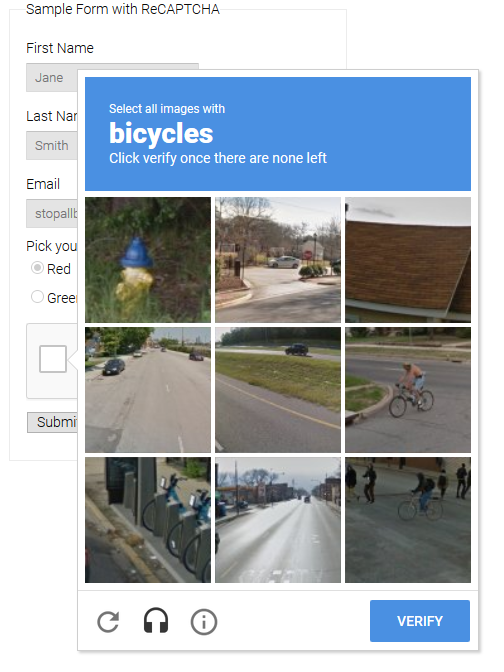
\includegraphics[scale=0.5]{recaptcha.png}
\caption{ReCaptcha Test von Google \cite{captchapic}}
\label{fig:recaptcha}
\end{wrapfigure}
Dabei sind die Antworten auf die eigentliche Frage nicht so wichtig wie es einem im ersten Moment erscheint. Die Ironie, und eine weitere Abweichung, ist dabei, dass man hier gegen ein neuronales Netzwerk "spielt". Dieses muss anhand der vorliegenden Informationen bestimmen, ob die Anfrage von einem Mensch stammt oder ob es sich dabei nur um eine automatisch generierte Anfrage handelt. Wie genau dieses Netzwerk entscheidet, weiß wahrscheinlich nicht mal Google. Wichtig ist aber, welche Daten dem Netzwerk dabei zur Verfügung gestellt werden, um seine Entscheidung zu treffen. Für weitere Informationen verweise ich hier auf einen Blog-Eintrag\cite{captcha}. Zu den auszuwertenden Daten gehören unter anderem die Mausbewegungen, sowie die gesendeten Daten des Browsers (z.B. User-Agent, IP, Cookies).
\subsection{Auswirkungen auf Kunst und Gesellschaft}
Diese grundsätzlichen Gedanken und die Frage, ob Maschinen überhaupt denken können, hat weitreichende Auswirkung auf die moderne Kunst, darunter vor allem Computerspiele. Sehr gute Beispiele sind das gleichnamige Spiel \textit{"The Turing Test"} oder auch \textit{"The Talos Principle"}, in denen der Turing Test sehr häufig vorkommt. In \textit{"The Turing Test"} geht es weiter folgend um die Fragen: Was ist wenn Mensch und Maschine im selben Körper sind? Hier wird ein klassischer textbasierter Turingtest eingesetzt, um Person und KI zu testen. Der Plot an dem ganzen Spiel ist, dass die Protagonistin nicht weiß, dass die KI teil von ihr ist und sie beeinflusst. Dieses Szenario erscheint erst einmal sehr kurios, wenn man aber einmal bedenkt, wie fortschrittlich unsere Implantattechnik bereits ist und wie diese weiter ausgebaut wird. In \textit{"The Talos Principle"} geht es um die Frage, ob wir Menschen nicht auch Maschinen sind und inwieweit Glauben, Neugier, und Unterhaltung uns von Maschinen abhebt. Deshalb ist die Frage "Was macht das mit uns Menschen und mit der KI" berechtigt. Es ist wichtig hier darauf aufmerksam zu machen, dass das Imitation Game heute noch für sehr viel Kopfzerbrechen unter den Wissenschaftlern, Philosophen, sowie in der gesamten Gesellschaft auslöst. Wir werden bald an den Zeitpunkt kommen wo es wichtig sein wird, sich mit dieser Frage auseinander zu setzen. Weiterführend dazu siehe "The future of the mind: Exploring machine consciousness" von Dr. Susan Schneider. \cite{explorecons}
